\documentclass[11pt]{article}
\usepackage[utf8]{inputenc}
\usepackage{booktabs}
\usepackage{multicol}
\usepackage{amsmath}
\usepackage{amsfonts}
\usepackage{fullpage}
\usepackage{amsmath,amssymb,amsthm}
\usepackage{tikz,lipsum,lmodern}
\usepackage[most]{tcolorbox}
\usepackage{graphicx}
\def\R{{\mathbb{R}}}
\def\N{{\mathbb{N}}}


\begin{center}
    
\includegraphics[width=17cm]{cover.png}
\end{center}

\newpage
\begin{document}
\section*{Abstract}
The purpose of this laboratory was to determine the efficiency when it came to the flywheel or the AC Generator. Understanding the power and energy transfer with an AC Generator. Investigating rotational kinetic energy with a flywheel. When finding the efficiency of the AC Generator, it provided an average of $55\%$. The explanation that was due to the conservation of energy, since the mass is being dropped from the pulley then there may have been kinetic energy between the string that was holding the mass and the pulley that was holding it. When the flywheel was put to the test, the efficiency was higher than the pulley. The average efficiency percentage of the flywheel was $59\%$, that could be due to the smoother surface of the flywheel.\\
Finally, when investigating the rotational kinetic energy with a flywheel, the inertia and angular velocity were found to determine the efficiency of the rotational kinetic energy. The efficiency calculated was $327\%$. That number is abnormally high but since we're calculating the efficiency of the rotational kinetic energy then there could be a factor that the kinetic energy between the flywheel and the A.C. Generator is high creating more energy than the pulley.

\section*{Introduction}
The purpose of the energy transfer experiment is to understand the power and energy transfer from an AC Generator and investigating the rotational kinetic energy from a flywheel. The energy transfer is used for demonstrating the energy conversion of stored gravitational potential energy into electrical energy. 
\begin{equation}
    P=\frac{V^2}{R}
\end{equation}
Where $P$ is the power from the energy transfer created by the AC Generator, $V$ is the voltage, and $R$ is the resistor of $100\Omega$. From the AC Generator there is a voltage output that must be created into power to determine how much power is created depending on the amount of weight, height difference there is.\\ To determine the difference between the power of the energy transfer from the AC Generator and the rotational kinetic energy from the flywheel, then efficiency will determine what provides more power. 
\begin{equation}
    \text{efficiency}=\frac{\text{energy generated}}{mgh}\cdot 100
\end{equation}
\begin{equation}
    \text{efficiency}=\frac{KE_{rot}}{mgh}\cdot 100
\end{equation}
Where $mgh$ is the potential energy from the distance of the pulley and the ground $h$, and the mass $m$ is from the string and weight. $KE$ is the rotational kinetic energy is determined by the rotational inertia $I$ and angular velocity $\omega$:
\begin{equation}
    KE_{rot}=\frac{1}{2}I\omega^2
\end{equation}
Moreover, the inertia is determined by the mass $m$ of the flywheel and the radius $R$ of the flywheel:
\begin{equation}
    I=\frac{1}{2}mR^2
\end{equation}


\section*{Procedure}
Refer to "Energy Transfer - Generator" instruction manual. The experiment followed the exact basic set up and procedure as the manual. This suggested experiments are the "Understanding Power and Energy Transfer with an AC Generator" and "Investigating Rotational Kinetic Energy with a Flywheel"

\section*{Data and Analysis}
The purpose of this laboratory is to understand the power and energy transfer, and investigating the rotational kinetic energy. By comparing both, it will determine the efficiency of both the ways of calculating power. The energy transfer is used for demonstrating the energy conversion of stored gravitational potential energy into electrical energy.\\
First, when trying to find the power and energy transfer from the AC Generator, it needs to have a source to start from. Meaning, when attaching a mass to the generator and dropping it; it allows for kinetic and potential energy to travel through the air, and make power. That being said, from the experiment there was a voltage output. From theory, equation (1), the voltage output is the voltage squared over resistor of power.
\begin{center}
    \textbf{Graph 1}: Instantaneous Power Generated from Voltage\\
    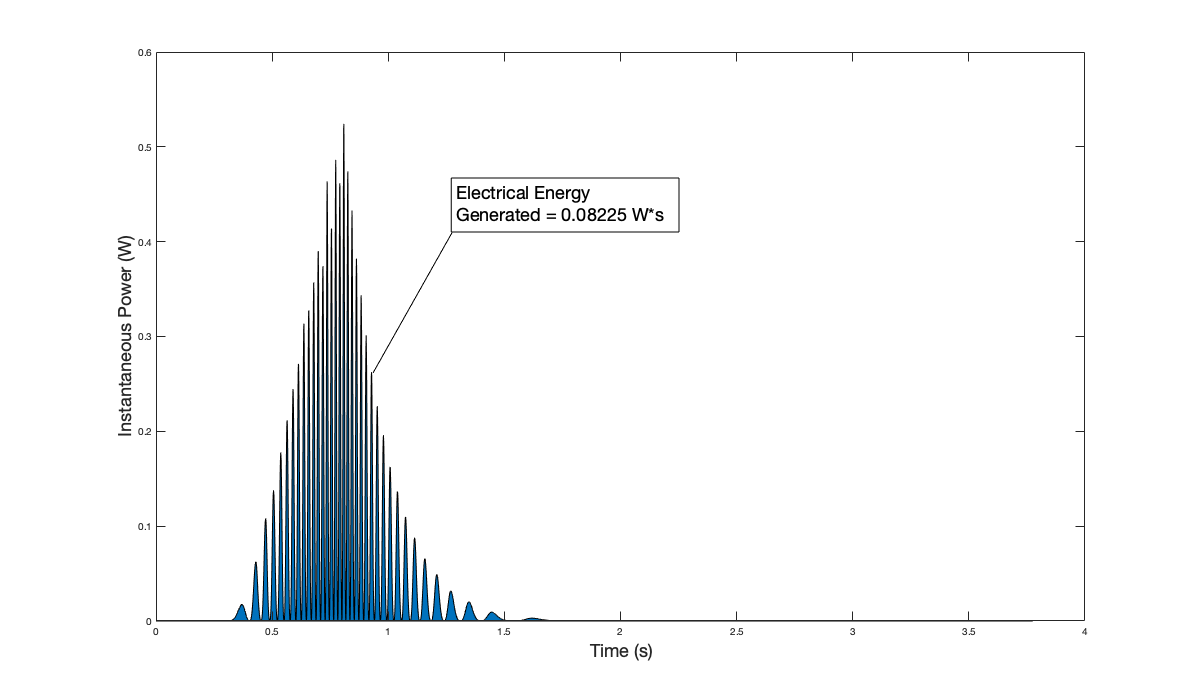
\includegraphics[width=17cm]{1.png}\\\textbf{Graph 1}: from the raw data collected, the graph was created through the calculations of equation (1). The independent value $x$ is the time measured in seconds. The dependent value $y$ is the instantaneous power measured in Watts. The area underneath the graph is the electrical energy generated being $0.082 W\cdot s$. This is an example of the graphs obtained through Capstone. 
\end{center}
From the instantaneous power graph comes the electrical energy generated if the integral of power is done. The electrical energy is found as an area underneath the power graph. The use of the electrical energy generated is to show the efficiency of the experiment. From the multiple calculated electrical energy generated in the Appendix table 1, the efficiency of the power and energy transfer from the AC generator is at an average of $54.7\%$. The rest of the energy is transferred into kinetic energy due to the law of conservation of energy. Meaning, that if multiple trials take place on the same pulley, there will be something called the "Thermal Pollution". Thus, most of the energy used is ultimately turned into heat. \\

\begin{center}
    \textbf{Graph 2}: Voltage Period for Angular Velocity\\
    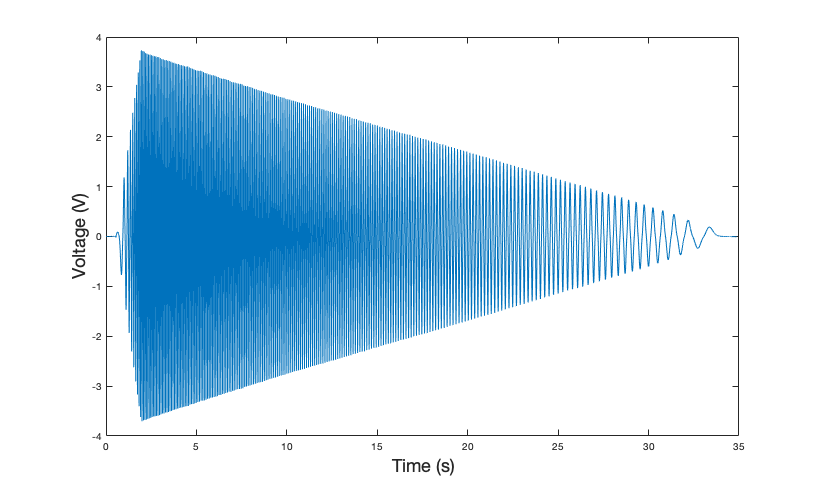
\includegraphics[width=17cm]{2.png}\\\textbf{Graph 2}: from the raw data collected, the graph was created through the calculations of equation (4). The independent value $x$ is the time measured in seconds. The dependent value $y$ is the voltage measured in volts. The period from this graph is used to determine the maximum angular frequency. To the determine the rotational kinetic energy. 
\end{center}
\\To test the efficiency of the flywheel, the same process was examined. Using equation (1), the voltage turns into power to be examined. For the most part, according to table 2 in the appendix the area underneath the power graph is consistent, and providing an efficiency percentage better than the AC generator. The average efficiency is at $59\%$. That could be due to the friction less surface from the flywheel, meaning that less energy is transferred to kinetic onto the pulley.\\
Furthermore, from measuring the period of the $A.C.$ voltage, it provided insight on the angular velocity. Based on equation (4), the kinetic energy is dependent on the angular velocity, which is needed to determine the maximum efficiency of the rotational kinetic flywheel. Since Inertia plays a role, the given information from the flywheel is the $79.1\pm0.005 g$ for mass and $6\pm 0.5cm$ for the radii. From the collected information, the maximum rotational kinetic energy is calculated. Also, the potential energy calculated was $0.14\pm0.0025 J$. Therefore, the efficiency of the maximum rotational wheel is about $327\%$ efficient. That could be due to the flywheel being friction less. To a point where the flywheel makes more energy then it is put in, that could mean that the fly wheel can create energy from the rotations that it is making.

\section*{Discussion and Conclusion}
To conclude, the purpose of this energy transfer experiment was to understand and investigate the efficiency of the rotational kinetic energy of a flywheel, and to understand the power and energy transfer with an AC Generator.\\
Firstly, with the help of equation (1), the instantaneous power was able to be calculated to determine the power created from the AC generator when the mass was dropped from the pulley. Nonetheless, the area under the instantaneous power gave an insight on the electrical energy generated, which was used to determine the efficiency of the AC Generator. The average efficiency was at $55\%$, due to most of the energy dissipating into kinetic energy on the friction between the cords and mass onto the pulley.\\
Secondly, when the flywheel was attached, the efficiency was better than the AC Generator even after following the exact process. The average efficiency was $59\%$. The reason why the efficiency is higher than the AC Generator is due to the smooth surface of the flywheel causing it to rotate longer and creating more energy.\\
Finally, when determining the rotational kinetic energy of the flywheel, with the help of equations (4) and (5). Equation (5) was calculated with the help of the flywheel by measuring the mass and the radius of the flywheel. Now that the inertia is determined, the angular velocity is missing from the equation. After finding the period of the A.C. voltage with the help of Capstone, the maximum angular frequency will be used to find the maximum rotational kinetic energy. After all the information for equation (3) is collected. The efficiency was found to be above $300\%$. The explanation behind such an increase is due to the flywheel collecting so much kinetic energy due to the spin that it creates more energy. 

\newpage
\section*{Appendix}
Wagih, Ghobriel: Lab manual I: Introduction to Experimental Physics.
\begin{center}
\caption{\textbf{Table 1}: Table of Information on Efficiency, Potential Energy, and Area} 
 \begin{tabular}{||c c c c c||} 
 \hline
 Area ($W\cdot s$) & Mass (g) & Height(cm) & Potential Energy (N) & Efficiency $\%$\\ [0.5ex] 
 \hline\hline
 0.08225 & $50\pm0.005$  & $30\pm0.5$ & $0.14715\pm0.00245$ & 55.895\\ 
 \hline
 0.08255 & - & - & - & 56.099 \\
 \hline
 0.08244 & - & - & - & 56.02\\
 \hline
 0.08053 & - & - & - & 54.73 \\
 \hline
 0.07813 & - & - & - & 53.095 \\
 \hline
 0.07920 & - & - & - & 53.82 \\
 \hline
 0.07809 & - & - & - & 53.07\\
 \hline
 0.08064 & - & - & - & 54.8\\
 \hline
 0.0763 & - & - & - & 51.85\\
 \hline
 0.0789 & - & - & - & 53.62 \\ [1ex] 
 \hline
\end{tabular}
\\\textbf{Table 1}: From the collected data, this table was made. The collected information is the Area, Mass, Height. Calculated information is the Potential Energy and Efficiency.
\end{center}
Calculation of Potential Energy:
\[PE=mgh=0.05\cdot 0.3\cdot 9.81=0.14715\pm 0.00245\]
Uncertainty of Potential Energy:
\[S_{PE}=\sqrt{\frac{S_m^2}{(m)^2}+\frac{S_h^2}{h^2}}0.14715=\sqrt{\frac{0.005^2}{0.3^2}+\frac{0.000005^2}{(0.05)^2}}\cdot 0.14715=0.00245254\]
\begin{center}
\caption{\textbf{Table 2}: Table of Information on Efficiency, Potential Energy, and Area} 
 \begin{tabular}{||c c c c c||} 
 \hline
 Area ($W\cdot s$) & Mass (g) & Height(cm) & Potential Energy (N) & Efficiency $\%$\\ [0.5ex] 
 \hline\hline
 0.08115 & $50\pm0.005$  & $28\pm0.5$ & $0.13734\pm0.00245$ & 59.08\\ 
 \hline
 0.08 & - & - & - & 58.2495 \\
 \hline
 0.08 & - & - & - & 58.2495\\
 \hline
 0.08 & - & - & - & 58.2495 \\
 \hline
 0.08 & - & - & - & 58.2495 \\
 \hline
 0.08 & - & - & - & 58.2495 \\
 \hline
 0.08 & - & - & - & 58.2495 \\
 \hline
 0.08 & - & - & - & 58.2495 \\
 \hline
 0.08443 & - & - & - & 61.475\\
 \hline
 0.08391 & - & - & - & 61.09 \\ [1ex] 
 \hline
\end{tabular}
\\\textbf{Table 2}: From the collected data, this table was made. The collected information is the Area, Mass, Height. Calculated information is the Potential Energy and Efficiency.
\end{center}
\newpage
\begin{center}
\caption{\textbf{Table 3}: Table of Information on Angular Velocity, Kinetic Energy, and Efficiency} 
 \begin{tabular}{||c c c c||} 
 \hline
 Inertia & Max Angular Velocity & Max Kinetic Energy (N) & Efficiency $\%$\\ [0.5ex] 
 \hline\hline
 $0.00014\pm 1.18\cdot10^{-5}$ & 79.49  & $0.45\pm 1.18\cdot10^{-5}$ & $327\%$\\ 
 \hline
 - & 79.49 & $0.45\pm 1.18\cdot10^{-5}$ & $327.5\%$\\
 \hline
 - & 80.51 & $0.46\pm 1.18\cdot10^{-5}$ & $335\%$\\
 \hline
 - & 79.49 & $$0.45\pm 1.18\cdot10^{-5}$$ & $327\%$ \\[1ex] 
 \hline
\end{tabular}
\\\textbf{Table 3}: From the collected data, this table was made. The collected information is the angular velocity, the calculated data is the Inertia, Max kinetic energy, and efficiency.
\end{center}
Calculation for Inertia and kinetic energy:
\[I=\frac{1}{2}mR^2=0.00014\]
\[KE=(\frac{1}{2})I\omega^2=0.45\]
Uncertainty on Inertia:
\[S_{I}=\sqrt{\frac{S_m^2}{(m)^2}+\frac{S_R^2}{R^2}}0.00014=\sqrt{\frac{0.005^2}{0.06^2}+\frac{0.000005^2}{(0.0791)^2}}\cdot 0.14715=0.00014\pm1.18\cdot10^{-5}\]

\end{document}